\documentclass[border=3mm]{standalone}
\usepackage{tikz}
\usetikzlibrary{circuits.logic.US}

\begin{document}
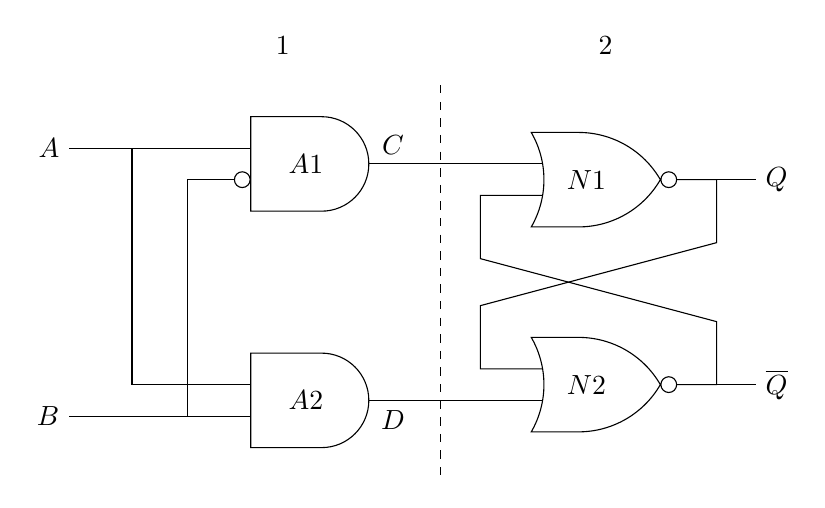
\begin{tikzpicture}[circuit logic US,
                    tiny circuit symbols,
                    every circuit symbol/.style={fill=white,draw,logic gate input sep=4mm, logic gate inverted radius=1mm}
]

% Draw the NOR gates
\node [nor gate, inputs = nn,info=center:$N1$] at (0,0) (nor1) {};
\node [nor gate, inputs = nn,info=center:$N2$] at ($(nor1.south)+(0cm,-2cm)$) (nor2) {};

% Draw the AND gates
%
\node
    % AND gate with one input inverted.
    [and gate, inputs = ni,info=center:$A1$]
    % Align AND gate output with nor1 input 1.
    at ($(nor1.input 1)+(-3,0)$) (and1) {};

\node
    % AND gate
    [and gate, inputs = nn,info=center:$A2$]
    % Align AND gate output with nor1 input 1.
    at ($(nor2.input 2)+(-3,0)$) (and2) {};

% AND gate inputs.
\draw (and1.input 1) -- ++(left:23mm) node[left] (A) {$A$};
\draw (and1.input 1) ++(left:15mm) |- (and2.input 1);
\draw (and2.input 2) ++(left:8mm) |- (and1.input 2);
\draw (and2.input 2) -- ++(left:23mm) node[left] (B) {$B$};

% Label AND gate outputs
\draw (and1.output) ++(right:3mm) node[above] {$C$};
\draw (and2.output) ++(right:3mm) node[below] {$D$};

% AND gate outputs are inputs to NOR1 input 1 and NOR2 input 2.
\draw (and1.output) |- (nor1.input 1);
\draw (and2.output) |- (nor2.input 2);

% Label NOR gate outputs.
\draw (nor1.output) -- ++(right:10mm) node[right] (U) {$Q$};
\draw (nor2.output) -- ++(right:10mm) node[right] (V) {$\overline{Q}$};

% Draw the NOR gate outputs back to respective inputs
%
% N1 output to N2 input 1.
\draw
    % Begin at N1 output
    (nor1.output)
    % zig-zag
    -- ++(right:5mm) -- ++(0,-8mm) -- ++(-3.0cm,-8mm )
    % to N2 input.
    |- (nor2.input 1);
%
% N2 output to N1 input 2.
\draw
    % Begin at N2 output
    (nor2.output)
    % zig-zag
    -- ++(right:5mm) -- ++(0,8mm) -- ++(-3.0cm,8mm )
    % to N1 input.
    |- (nor1.input 2);

% Label regions. Dashed line and number regions.
\draw ($(and1.output)+(9mm,1)$)[dashed] -- ++(270:5);
\draw ($(and1.output)+(-11mm,1.5)$) node {1};
\draw ($(and1.output)+(30mm,1.5)$) node {2};

\end{tikzpicture}
\end{document}
